\chapter{Results}
\label{chapter:results}

\section{Stage 1: a small synthetic offset}
\label{sec:results-stage1}

The first PPO run on stage 1's original (tight) tolerance achieved 0/20 success. Following the
project's diagnostic protocol -- does a naive baseline solve it, is the shaped potential
decreasing, does the terminal bonus ever fire, does loosening the tolerance $10\times$ help --
a traced episode showed the policy closing to $\sim$\SI{650000}{km}/\SI{200}{m/s} around day 250,
then drifting past the target and diverging by day 400. This is a direct consequence of
$\gamma=1$ potential-based shaping: since the shaping reward telescopes to the \emph{net}
start-to-end change, it gives no incentive to loiter near the target once close, only to have
been close at some point. Re-evaluating the same trained checkpoint with the tolerance loosened
$10\times$ (no retraining) succeeded immediately, at day 217 -- confirming the reward and policy
were both fine, and the tolerance had simply been tighter than achievable within the training
budget. Retraining stage 1 at the loosened tolerance (\SI{1e6}{km}/\SI{500}{m/s}) for
1{,}000{,}000 steps reaches 20/20 deterministic success, clearly separated from both baselines
(Figure~\ref{fig:stage1-curve}).

\begin{figure}[H]
  \centering
  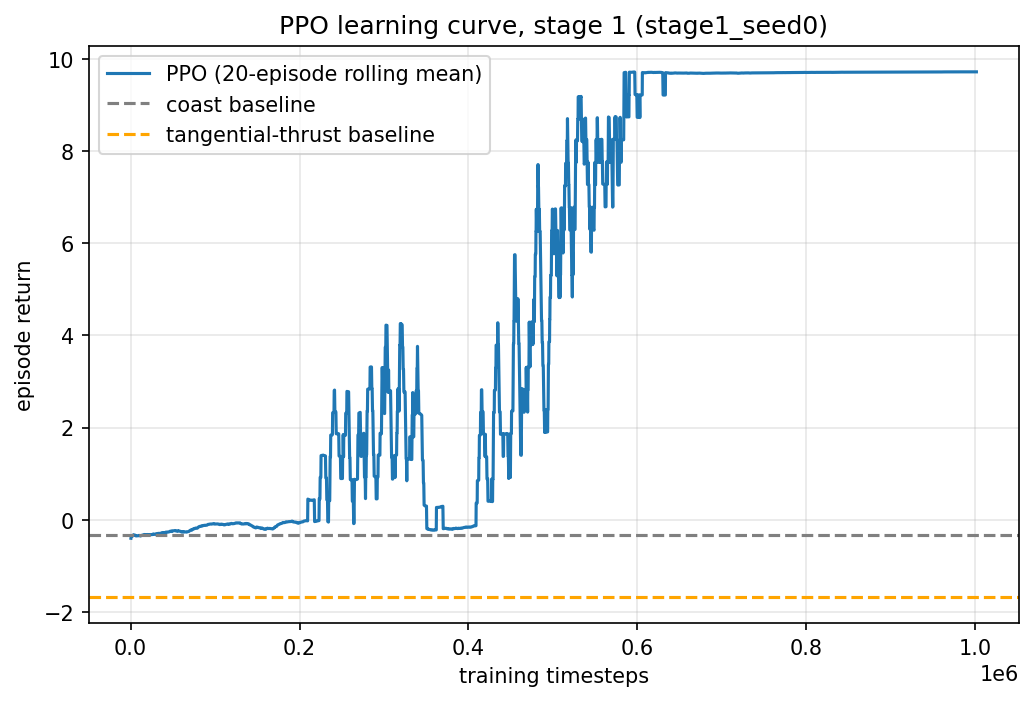
\includegraphics[width=0.8\textwidth]{figures/learning_curve_stage1_seed0.png}
  \caption{Stage-1 learning curve (single seed) against the coast and tangential-thrust
    baselines.}
  \label{fig:stage1-curve}
\end{figure}

\section{Stage 2: a larger synthetic offset}
\label{sec:results-stage2}

Stage 2 combines a semi-major-axis offset five times larger than stage 1 with a $2\deg$
inclination change. Four different fixes were attempted, each targeting a specific hypothesis for
the failure, and none succeeded:
\begin{enumerate}
  \item Warm-started from stage 1, original tight tolerance: 0/5 success, return drifting worse.
  \item From scratch (ruling out a stale, low-exploration warm-started policy), tolerance
        loosened $10\times$ as in stage 1: still 0/5, $\lVert\Delta\vec r\rVert$ plateaued around
        110--145 million km for the whole run.
  \item Time window extended 400$\to$600 days (raising the delta-v budget directly, rather than
        loosening tolerance again): still failed,
        $\lVert\Delta\vec r\rVert\sim$190--220 million km, worse than the 400-day coast baseline
        in absolute terms.
  \item Warm-started from stage 1 with exploration noise manually reset
        ($\mathrm{std}: 0.235\to1.0$, ruling out exploration collapse specifically): still failed,
        $\mathrm{ep\_rew\_mean}=-2.25$.
\end{enumerate}
Stage 2's delta-v margin (Section~\ref{sec:reachability}'s method applied to its own target) is
only $1.2\times$ the available budget -- tight enough that an imperfect learned policy may simply
not have the fuel margin to correct a suboptimal early trajectory. This is treated as a genuine,
documented open finding rather than a bug: the combined $\Delta a + \Delta i$ maneuver may need
something other than greedy potential-based shaping, which can locally mislead a policy into
directly closing distance instead of executing a more efficient indirect transfer.

\section{Final configuration: randomised real asteroids}
\label{sec:results-final}

Per the project plan's own priority order, the final multi-seed randomised-target configuration
(warm-started from stage 1, not stage 2) was trained regardless of stage 2's outcome: 5
independent seeds, 1{,}000{,}000 steps each, target and time window resampled every episode from
the delta-v-feasibility pool of real GTOC4 asteroids (Section~\ref{sec:reachability}).

\begin{table}[H]
  \centering
  \caption{Deterministic evaluation (20 episodes/seed, unseen targets) of the final randomised
    configuration, against baselines averaged over 10 sampled targets.}
  \label{tab:randomised-results}
  \begin{tabular}{lcc}
    \toprule
    Configuration & Success rate & Mean return \\
    \midrule
    PPO, seed 1--5 & 0/20 (all 5 seeds) & $-1.79$ to $-2.10$ \\
    Coast baseline & -- & $-1.79 \pm 1.25$ \\
    Tangential-thrust baseline & -- & $-5.10 \pm 1.24$ \\
    \bottomrule
  \end{tabular}
\end{table}

All 5 seeds fail (0/20), and their mean returns are statistically indistinguishable from simply
coasting, while still beating the actively wasteful tangential-thrust baseline
(Figure~\ref{fig:randomised-curve}). In other words, the policy reliably learned \emph{not to
waste propellant}, but not to rendezvous. This mirrors stage 2's failure and is consistent with
it: the randomised task combines stage 2's unsolved $\Delta a + \Delta i$ problem with real
asteroids over multi-year windows -- strictly harder, not easier, than stage 2.

\begin{figure}[H]
  \centering
  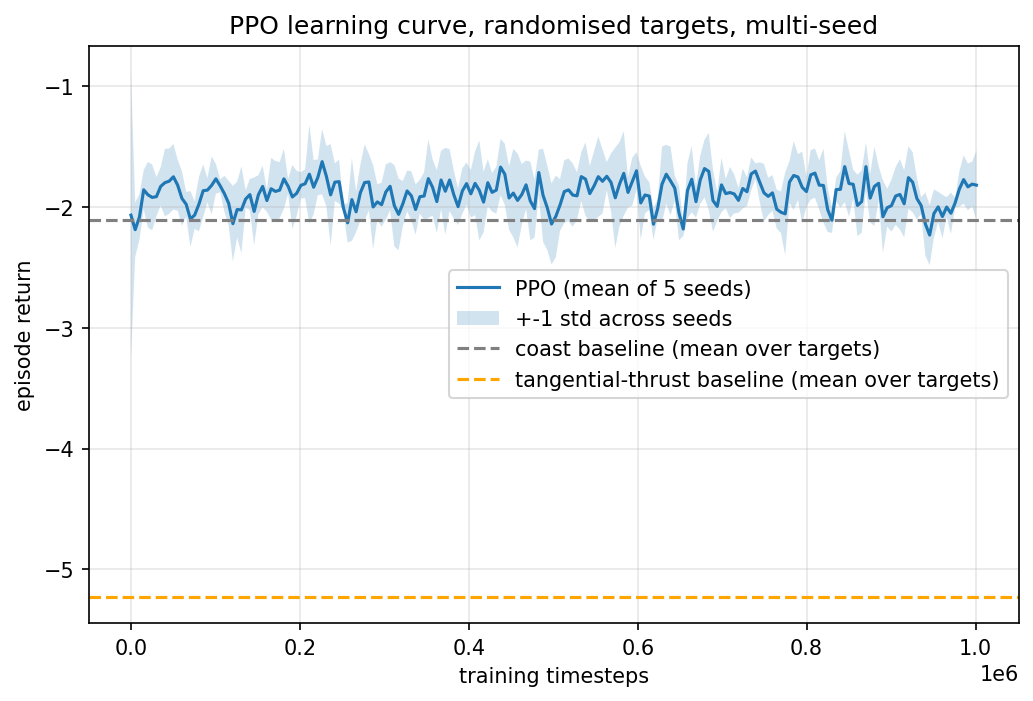
\includegraphics[width=0.8\textwidth]{figures/learning_curve_randomized_multiseed.png}
  \caption{Multi-seed learning curve (mean $\pm$ std over 5 seeds) for the final randomised
    configuration, against baseline reference lines.}
  \label{fig:randomised-curve}
\end{figure}

\section{Sensitivity analysis}
\label{sec:wp6}

Five environment/reward knobs were swept one-at-a-time around the stage-1 baseline configuration
(control interval, position tolerance, velocity tolerance, propellant penalty, rendezvous bonus),
3 values $\times$ 3 seeds each, at half the stage-1 training budget (500{,}000 steps, to keep 33
runs tractable). This budget cut turned out to matter: the baseline configuration itself, which
reaches 20/20 at 1{,}000{,}000 steps, only reaches 0/20 at 500{,}000 -- its return is still
climbing steeply at that point (Section~\ref{sec:results-stage1}). The sweep should therefore be
read as showing which changes let \emph{some} success appear within a fixed, sub-convergence
budget, not as a sensitivity of fully-converged performance.

\begin{table}[H]
  \centering
  \caption{Sensitivity sweep results (success rate, mean over 3 seeds). Bold: the shared stage-1
    baseline value for that parameter.}
  \label{tab:sensitivity}
  \begin{tabular}{lccc}
    \toprule
    Parameter & Looser/easier value & Baseline & Tighter/harder value \\
    \midrule
    Control interval (days) & 2: 0.33 & \textbf{1: 0.00} & 0.5: 0.00 \\
    Position tolerance (km) & $10^7$: 1.00 & \textbf{$10^6$: 0.00} & $10^5$: 0.00 \\
    Velocity tolerance (m/s) & 2000: 0.33 & \textbf{500: 0.00} & 100: 0.00 \\
    Propellant penalty & 0.01: 0.00 & \textbf{0: 0.00} & 0.05: 0.00 \\
    Rendezvous bonus & 2: 0.00 & \textbf{10: 0.00} & 30: 0.00 \\
    \bottomrule
  \end{tabular}
\end{table}

Under this reduced budget, only changes that make the task \emph{easier per unit of experience}
-- a looser tolerance, or a coarser control interval requiring fewer sequential decisions per
mission -- recover any success at all (Figure~\ref{fig:sensitivity-example}); propellant penalty
and rendezvous bonus, which do not change how hard the underlying transfer is, have no effect
within budget. This is itself a useful (if unplanned) finding about the interaction between task
difficulty and the compute budget needed for PPO to converge on this problem, though a full-budget
re-run would be needed to characterise sensitivity of the \emph{converged} policy.

\begin{figure}[H]
  \centering
  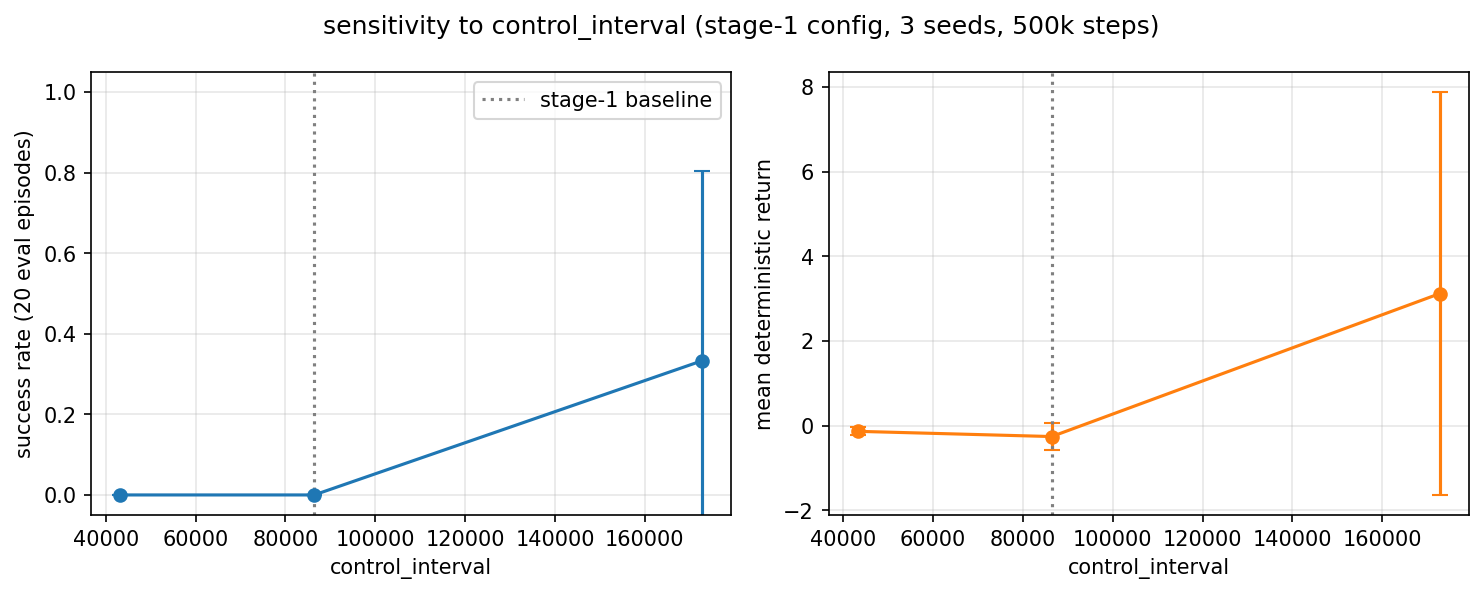
\includegraphics[width=\textwidth]{figures/sensitivity_control_interval.png}
  \caption{Sensitivity to control interval: success rate and mean return vs.\ value (mean
    $\pm$ std over 3 seeds).}
  \label{fig:sensitivity-example}
\end{figure}

\section{Learned controller analysis}
\label{sec:wp7}

This section analyses the one policy that did converge: the stage-1 checkpoint from
Section~\ref{sec:results-stage1}.

\paragraph{Thrust profile and bang-bang structure.} Over a full successful rollout (114 days),
throttle is at 100\% for every single control step (Figure~\ref{fig:thrust-profile},
\ref{fig:bang-bang}): the learned controller is bang-bang in the trivial, degenerate sense of
always thrusting at maximum -- it never coasts at all, only steers thrust direction. This is
consistent with mass/time-optimal low-thrust control theory (which predicts thrust-on except
possibly for short coast arcs), but the complete absence of any coast phase suggests the transfer
found here is closer to a minimum-time solution for this specific, short, easy target than a
finely-tuned mass-optimal one.

\begin{figure}[H]
  \centering
  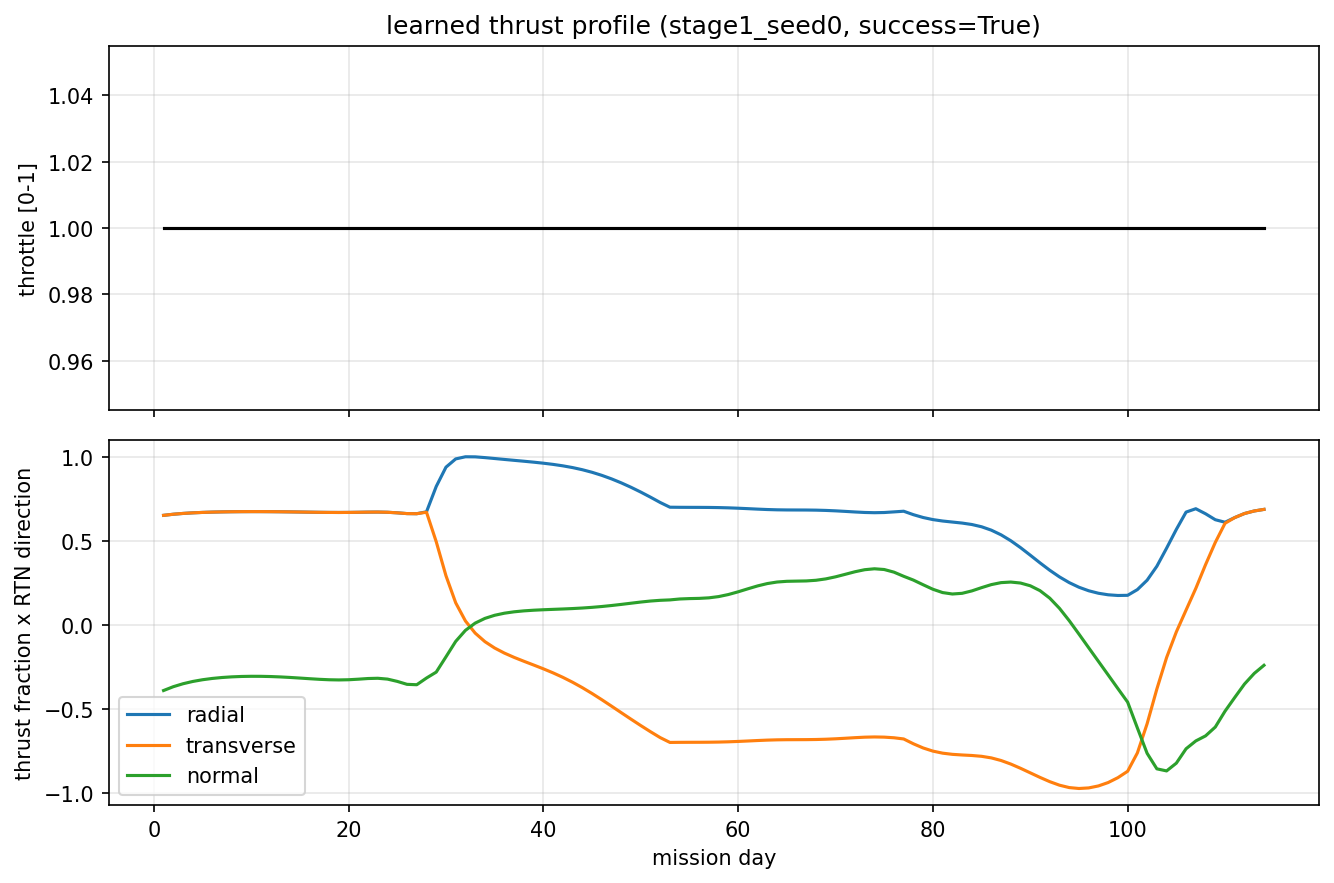
\includegraphics[width=0.85\textwidth]{figures/wp7_thrust_profile.png}
  \caption{Throttle and RTN thrust direction components over one successful stage-1 rollout.}
  \label{fig:thrust-profile}
\end{figure}

\begin{figure}[H]
  \centering
  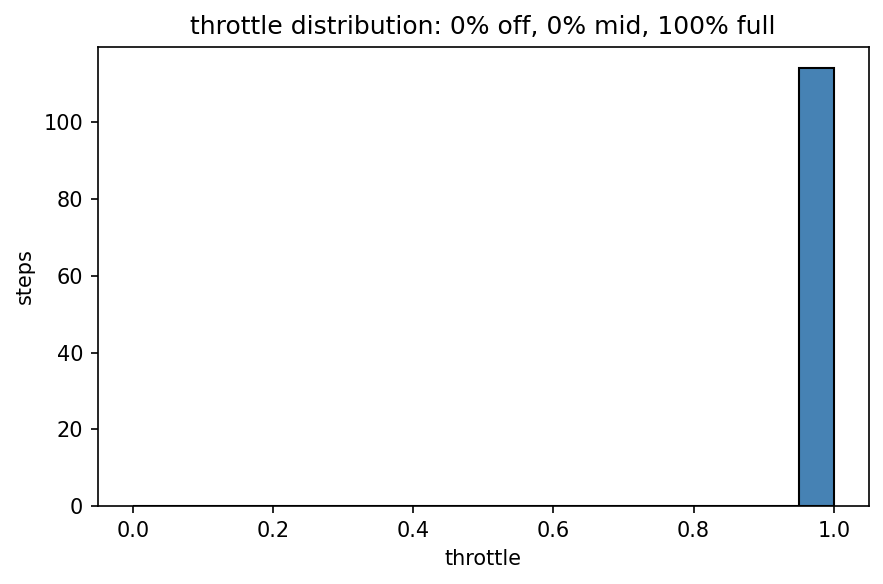
\includegraphics[width=0.55\textwidth]{figures/wp7_bang_bang_histogram.png}
  \caption{Throttle distribution over the same rollout: 100\% of steps at full throttle.}
  \label{fig:bang-bang}
\end{figure}

\paragraph{Policy probing.} The policy was fed synthetic observations with $\Delta\vec r$ rotated
through 8 directions at fixed magnitude around an otherwise fixed ``mid-mission, on-track'' state.
The commanded thrust direction and throttle were nearly identical across all 8 probe angles
(differences only in the third decimal place; Figure~\ref{fig:policy-probe}) -- the policy is
essentially \emph{insensitive} to the direction of the position error at this synthetic state.
Combined with the failure-mode result below, this suggests the stage-1 policy has not learned a
general closed-loop ``point thrust to close the gap'' rule, but something closer to a fixed,
(roughly) time-indexed maneuver tuned to its one training geometry.

\begin{figure}[H]
  \centering
  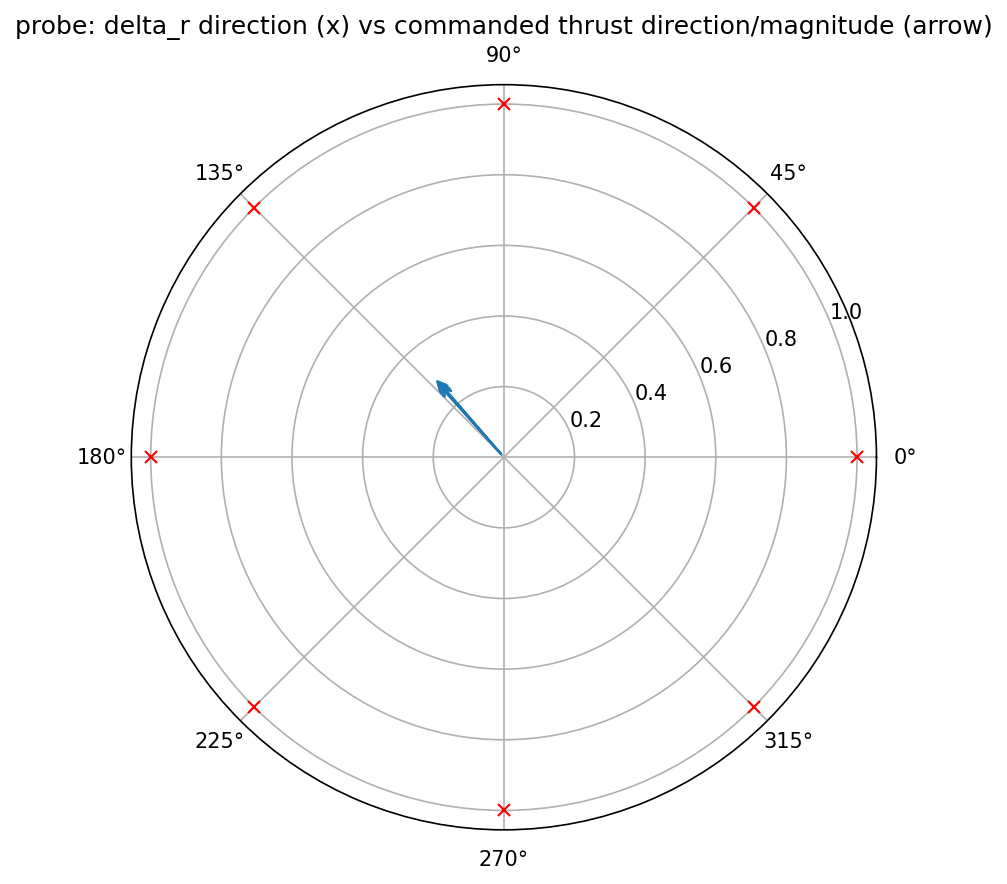
\includegraphics[width=0.55\textwidth]{figures/wp7_policy_probe.png}
  \caption{Commanded thrust direction/magnitude (arrows) for 8 synthetic $\Delta\vec r$
    directions (red $\times$): all responses cluster together, regardless of probe angle.}
  \label{fig:policy-probe}
\end{figure}

\paragraph{Failure-mode sweep.} Without any retraining, the stage-1 policy was evaluated (10
episodes each) against targets with $\Delta a$ swept from its trained value ($0.02\,\mathrm{AU}$) up to
stage 2's ($0.1\,\mathrm{AU}$). Success collapses from 10/10 to 0/10 the moment $\Delta a$ is doubled
(Figure~\ref{fig:failure-sweep}) -- a sharp cliff exactly at the training distribution's edge,
reinforcing the ``memorised one geometry'' picture above.

\begin{figure}[H]
  \centering
  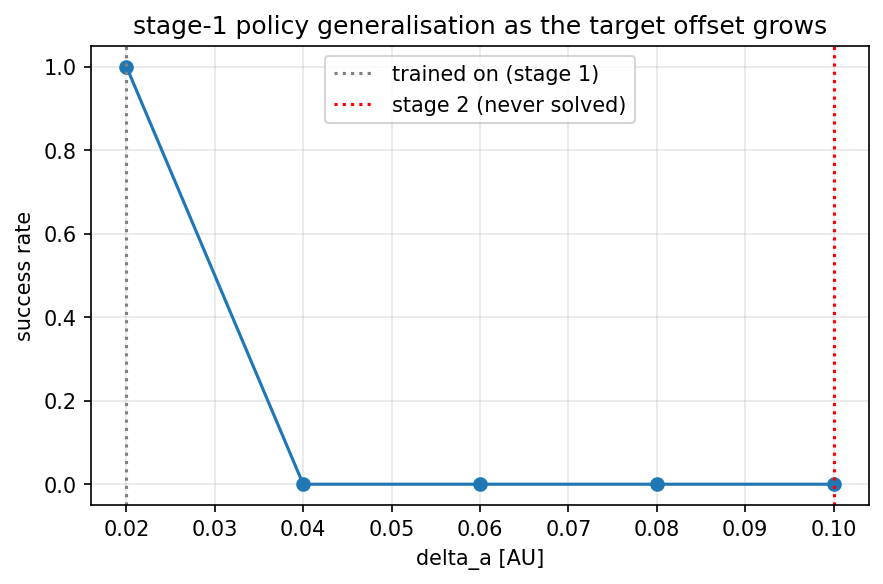
\includegraphics[width=0.7\textwidth]{figures/wp7_failure_sweep.png}
  \caption{Stage-1 policy success rate as the target's semi-major-axis offset grows beyond its
    training value.}
  \label{fig:failure-sweep}
\end{figure}

\paragraph{Mass-optimality gap.} Comparing the learned policy's propellant use to a closed-form
impulsive delta-v lower bound (Section~\ref{sec:reachability}'s estimate applied to the stage-1
target): the lower bound is \SI{835.4}{m/s}; the learned policy's equivalent delta-v (via the
rocket equation on its actual mass used) is \SI{900.1}{m/s} -- a $+7.7\%$ gap. For a continuous-
thrust policy against an idealised impulsive lower bound, this is a small and reasonable gap,
and is itself evidence that the trained policy is not simply routing to the target
inefficiently.

\begin{figure}[H]
  \centering
  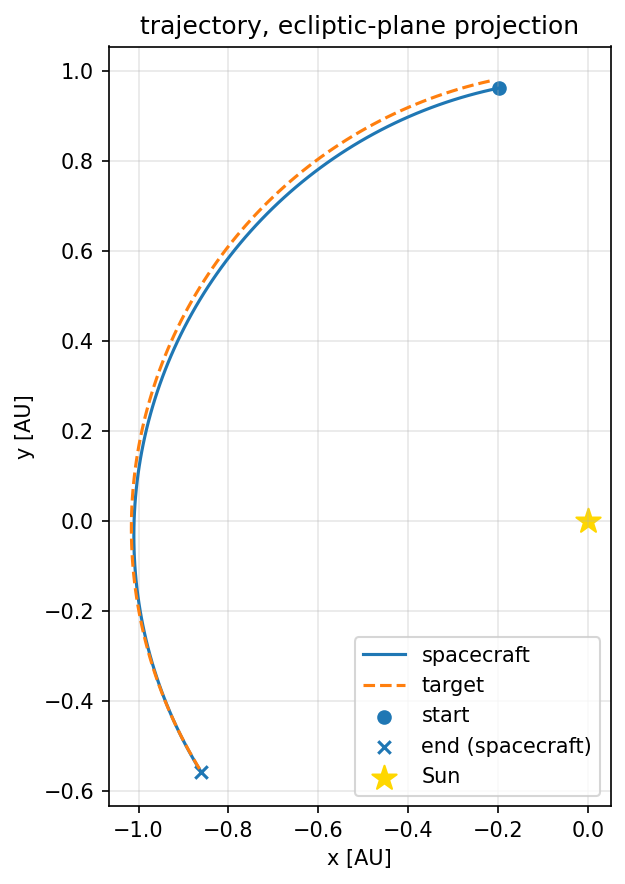
\includegraphics[width=0.7\textwidth]{figures/wp7_trajectory.png}
  \caption{Ecliptic-plane projection of the same rollout: spacecraft trajectory closely tracks
    the target's orbit and converges onto it.}
  \label{fig:trajectory}
\end{figure}

\section{Independent verification under Tudat}
\label{sec:wp8}

The exact thrust command history from the stage-1 rollout above (piecewise-constant direction and
magnitude, one segment per control day) was replayed through Tudat's adaptive RKF78 integrator,
independent of the fixed-step RK4 propagator used during training, to check whether the learned
control law is a real physical solution or an artifact of RK4's specific numerical behaviour.

\begin{table}[H]
  \centering
  \caption{Final rendezvous state: RK4 (training) vs.\ Tudat replay of the identical thrust
    history. Stage-1 tolerance: \SI{1e6}{km} / \SI{500}{m/s}.}
  \label{tab:tudat-verify}
  \begin{tabular}{lccc}
    \toprule
    Propagator & $\lVert\Delta\vec r\rVert$ (km) & $\lVert\Delta\vec v\rVert$ (m/s) & Final mass (kg) \\
    \midrule
    RK4 (training) & 973{,}241 & 488.1 & 1454.8 \\
    Tudat (RKF78, independent) & 869{,}949 & 480.1 & 1453.8 \\
    \bottomrule
  \end{tabular}
\end{table}

Both propagators agree the rendezvous condition is met, with final position/velocity/mass within
$\sim$10\%/1.6\%/0.07\% of each other -- larger than the few-meter agreement found for an
uncontrolled coast in Section~\ref{sec:dynamics}, as expected given error accumulates over 114
days of a thrust-steered trajectory rather than a single ballistic arc, but small relative to the
tolerance itself. The learned policy's success generalises to an independent, higher-fidelity
integrator: it is a real physical solution, not an RK4-specific artifact.
